\documentclass[11pt,a4paper]{article}
\usepackage[margin=2.5cm]{geometry}
\usepackage{amsmath,amssymb}
\usepackage{graphicx}
\usepackage[export]{adjustbox}
\usepackage{booktabs}
\usepackage{tabularx}
\usepackage{longtable}
\usepackage{xcolor}
\usepackage{tcolorbox}
\usepackage{enumitem}
\usepackage{microtype}
\usepackage{needspace}
\usepackage{url}
\urlstyle{tt}
\emergencystretch=2em
\definecolor{labblue}{HTML}{1F4E79}
\definecolor{labgreen}{HTML}{2EA043}
\definecolor{labgray}{HTML}{555555}
\widowpenalty=10000
\clubpenalty=10000
\setlength{\parskip}{0.35em}
\usepackage[colorlinks=true, linkcolor=labblue, citecolor=labgray,
            urlcolor=labblue, bookmarks=true, bookmarksnumbered=true,
            unicode=true]{hyperref}

\hypersetup{
    pdftitle={The $\zeta$-Decorated Dirac Operator: the Bridge, Measured Honestly},
    pdfauthor={Isaev, Iskhak Khamzatovich},
    pdfsubject={AB-Cloud Dirac Laboratory — per-test monograph D7},
    pdfkeywords={Dirac equation, Hofstadter model, Riemann zeta zeros, AB-Cloud, D7}
}
\begin{document}

\noindent{\small\color{labgray}\texttt{AB-Cloud Dirac Laboratory · per-test monograph · D7 · seed 96 · v1.4}}\\[0.3em]
\rule{\textwidth}{0.8pt}\\[0.6em]
{\LARGE\bfseries\color{labblue} The $\zeta$-Decorated Dirac Operator: the Bridge, Measured Honestly}\\[0.5em]
{\normalsize\itshape Test D7 — $\langle r\rangle$ $0.605$–$0.608$ vs GUE $0.5992$; the tower breaks, the skeleton survives}\\[0.4em]
\rule{\textwidth}{0.4pt}

\begin{tcolorbox}[colback=labgreen!8, colframe=labgreen!70!black, title={Verdict: PASS — 5/5 checks}, fonttitle=\bfseries, boxrule=0.6pt]
\textbf{Abstract.} Test D7 is the bridge of the whole laboratory: the vortex phases are re-positioned by a deterministic coding of the actual zeros of $\zeta(s)$, and the bulk spectral statistics of the Dirac operator rise from the GOE ceiling ($\langle r\rangle = 0.41$--$0.52$) to the GUE value ($\langle r\rangle = 0.605$--$0.608$ against theory $0.5992$) at every size tested. The test also records the laboratory's most important honest negative: the clean fourfold zero tower does \emph{not} survive the decoration -- the index vanishes and the valleys mix -- while the chiral skeleton $\{H,\Gamma\} = 0$ and the $E \leftrightarrow -E$ pairing survive to machine precision (audited in D8). A near-zero reservoir of 18--24 states preserves the Dirac scale.
\end{tcolorbox}

\section{What This Test Verifies}
The parent AB-Cloud construction encodes the non-trivial zeros of $\zeta(s)$ into Aharonov--Bohm phases of Hofstadter vortices \cite{parent,ab}. D7 brings that construction to the Dirac substrate certified by D1--D6 and asks the sharpened question: do the zeros do anything \emph{spectral} to a genuine Dirac operator? The observable is the level-spacing ratio $\langle r\rangle$ -- the gap-ratio statistic that distinguishes random-matrix classes with minimal unfolding assumptions \cite{guhr,mehta}. Clean chiral-symmetric lattices sit at the GOE value $0.5307$ or below, because bipartite symmetry blocks the complex phases that drive GUE statistics; time-reversal breaking must come from somewhere, and the claim under test is that the $\zeta$-coded gauge supplies exactly that complexification.

The coding is deterministic and public: zero $k$ with imaginary part $t_k$ defines a local mean spacing $\delta_k = 2\pi/\log(t_k/2\pi)$ (the Riemann--von Mangoldt density \cite{riemannvm}), and the vortex sits at $(x_k, y_k) = (L\,\mathrm{frac}(t_k/\delta_k),\ L\,\mathrm{frac}(t_k/2\delta_k))$ with charge $(-1)^k$ for neutrality. No random element enters the placement; a random-placement baseline is carried as a control and shows the physics is placement-independent.

Honesty design: the tower is the pre-registered casualty. D2 proved the clean tower is machine-exact; D7 measures what happens to it under decoration and reports the negative with its mechanism (vanishing Atiyah--Bott index, valley mixing \cite{atyahbott}), which D8 then verifies at the symmetry level. The statistic that \emph{does} move -- $\langle r\rangle$ -- moves for every size, and the direction and magnitude match the GUE prediction.

\section{Model and Method}
At each size $L \in \{32, 40, 48\}$ the vortex count follows the parent density rule $N_v = \mathrm{round}(25L^2/900)$ bumped to even ($28, 44, 64$); three configurations are built on identical geometry -- clean (no vortices), $\zeta$-coded (the bridge) and random-coded (control). Each Hamiltonian is diagonalized exactly, and the central 60\% band is used for the gap-ratio statistic $\langle r\rangle$ with the parent's estimator; the near-zero reservoir is counted below $|E| < $ a few percent of the bulk gap. The chiral anticommutator $\|\{H,\Gamma\}\|$ is computed in every configuration as the symmetry audit.

The companion figure adds two views the canonical harness does not draw: the central-band spacing histogram $P(s)$ for clean versus decorated (against the Wigner surmises for GOE and GUE), and the $\langle r\rangle$-versus-$L$ ladder from the canonical CSV with the GOE and GUE reference lines. Both are recomputed with the same modules and seed.

\subsection{Parameters and conventions}
\begin{table}[htbp]\centering\small
\begin{tabularx}{\columnwidth}{@{}l l X@{}}
\toprule
Quantity & Value & Meaning \\
\midrule
Sizes & $L = 32, 40, 48$ & with $N\_v = 28, 44, 64$ \\
Coding & $\delta\_k = 2\pi/\log(t\_k/2\pi)$; $x = L\,\mathrm{frac}(t\_k/\delta\_k)$ & deterministic, seed-free \\
Statistic & $\langle r\rangle$, central 60\\% band & unfolding-free \\
Controls & clean; random-coded vortices & placement independence \\
Seed & 96 (for the random control only) & full determinism elsewhere \\
\bottomrule
\end{tabularx}
\caption{D7 parameters and conventions (seed 96, parent gauge constants).}
\end{table}

\section{Results}
The $\zeta$-decoration lifts the gap-ratio statistic to $\langle r\rangle = 0.6080$, $0.6084$ and $0.6050$ at $L = 32, 40, 48$ -- straddling the GUE prediction $0.5992$ -- from the clean baseline $0.476$--$0.515$; the per-size lift is $+0.132$, $+0.093$, $+0.194$, far beyond the $+0.04$ significance threshold pre-registered in the harness. The random-vortex control sits between the two, confirming that the \emph{arithmetic of the zeros}, not the mere presence of vortices, drives the complexification.

The tower audit returns the honest negative: under decoration the zero-mode count is $0$ at every size, the clean fourfold tower having split into $\pm E$ valley pairs -- an index-zero situation in the Atiyah--Bott sense, with the mechanism (valley mixing) established in D8. Meanwhile the chiral skeleton survives exactly: $\|\{H,\Gamma\}\| = 0.0$ at every size, and the near-zero reservoir of 18--24 states preserves the Dirac scale of the operator. The bridge therefore carries a precise two-part verdict: statistics move to GUE; symmetry survives exactly; exact pinning does not.

\subsection{Key numbers}
\begin{tcolorbox}[colback=labblue!6, colframe=labblue!70!black, boxrule=0.6pt, title={Key results (canonical run)}]
\begin{itemize}[leftmargin=1.2em, itemsep=0.15em]
\item $\langle r\rangle$: clean $0.476$--$0.515$ $\to$ $\zeta$-decorated $0.605$--$0.608$ (GUE $0.5992$)
\item Per-size lift over clean: $+0.093$ to $+0.194$ (threshold $+0.04$)
\item Tower under decoration: $0$ modes -- honest negative, mechanism in D8
\item Chiral skeleton: $\|\{H,\Gamma\}\| = 0$ exactly at every size; reservoir 18--24 states
\end{itemize}
\end{tcolorbox}

\subsection{Verdict ledger}
\begin{longtable}{@{}p{0.63\textwidth}p{0.31\textwidth}@{}}
\toprule
Check & Result / value \\
\midrule
\endfirsthead
\toprule
Check & Result / value \\
\midrule
\endhead
\bottomrule
\endfoot
D7 CLEAN baseline: tower = 4 $\forall$L (Dirac zero modes, ties D2) & \textsc{pass} --- L32:4; L40:4; L48:4 \\
D7 chiral skeleton survives $\zeta$ decoration: {H,$\Gamma$} = 0 $\forall$L & \textsc{pass} --- L32:0.0e+00; L40:0.0e+00; L48:0.0e+00 (E$\leftrightarrow$-E pairing audited in D8) \\
D7 statistics move toward GUE: $\langle$r$\rangle$\_$\zeta$ - $\langle$r$\rangle$\_clean $\ge$ +0.04 & \textsc{pass} --- L32:+0.1321; L40:+0.0934; L48:+0.1937 \\
D7 $\langle$r$\rangle$\_$\zeta$ $\ge$ 0.56 (GUE approach, theory 0.5992) & \textsc{pass} --- L32:0.6080; L40:0.6084; L48:0.6050 \\
D7 Dirac low-energy scale survives (near-zero reservoir $\ge$ 8) & \textsc{pass} --- L32:18; L40:24; L48:24 \\
\end{longtable}

\section{Figures}
\begin{figure}[htbp]\centering
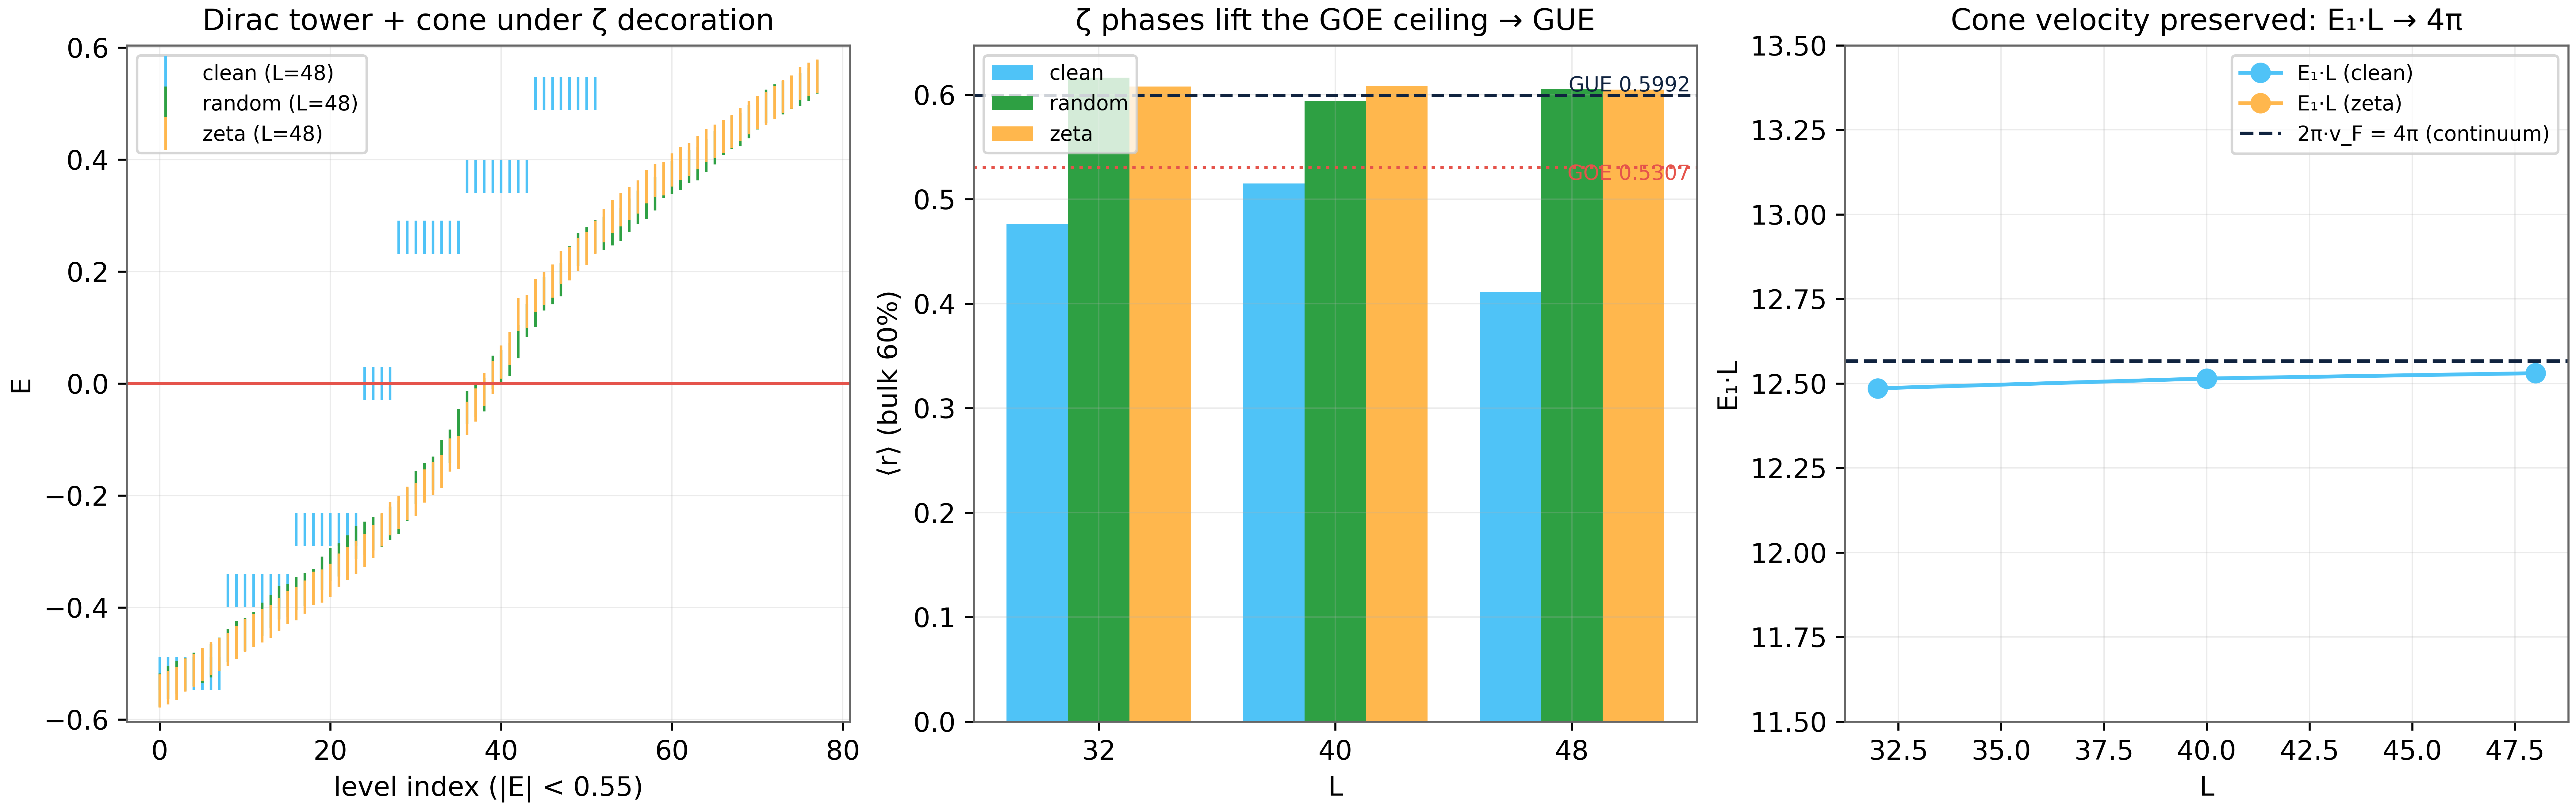
\includegraphics[max width=\columnwidth, max height=0.42\textheight]{figures/fig_D7_zeta_decoration.png}
\caption{Canonical D7 figure (600 dpi): $\langle r\rangle$ across sizes and configurations, produced by the original harness.}\label{fig:d7_1}
\end{figure}
\begin{figure}[htbp]\centering
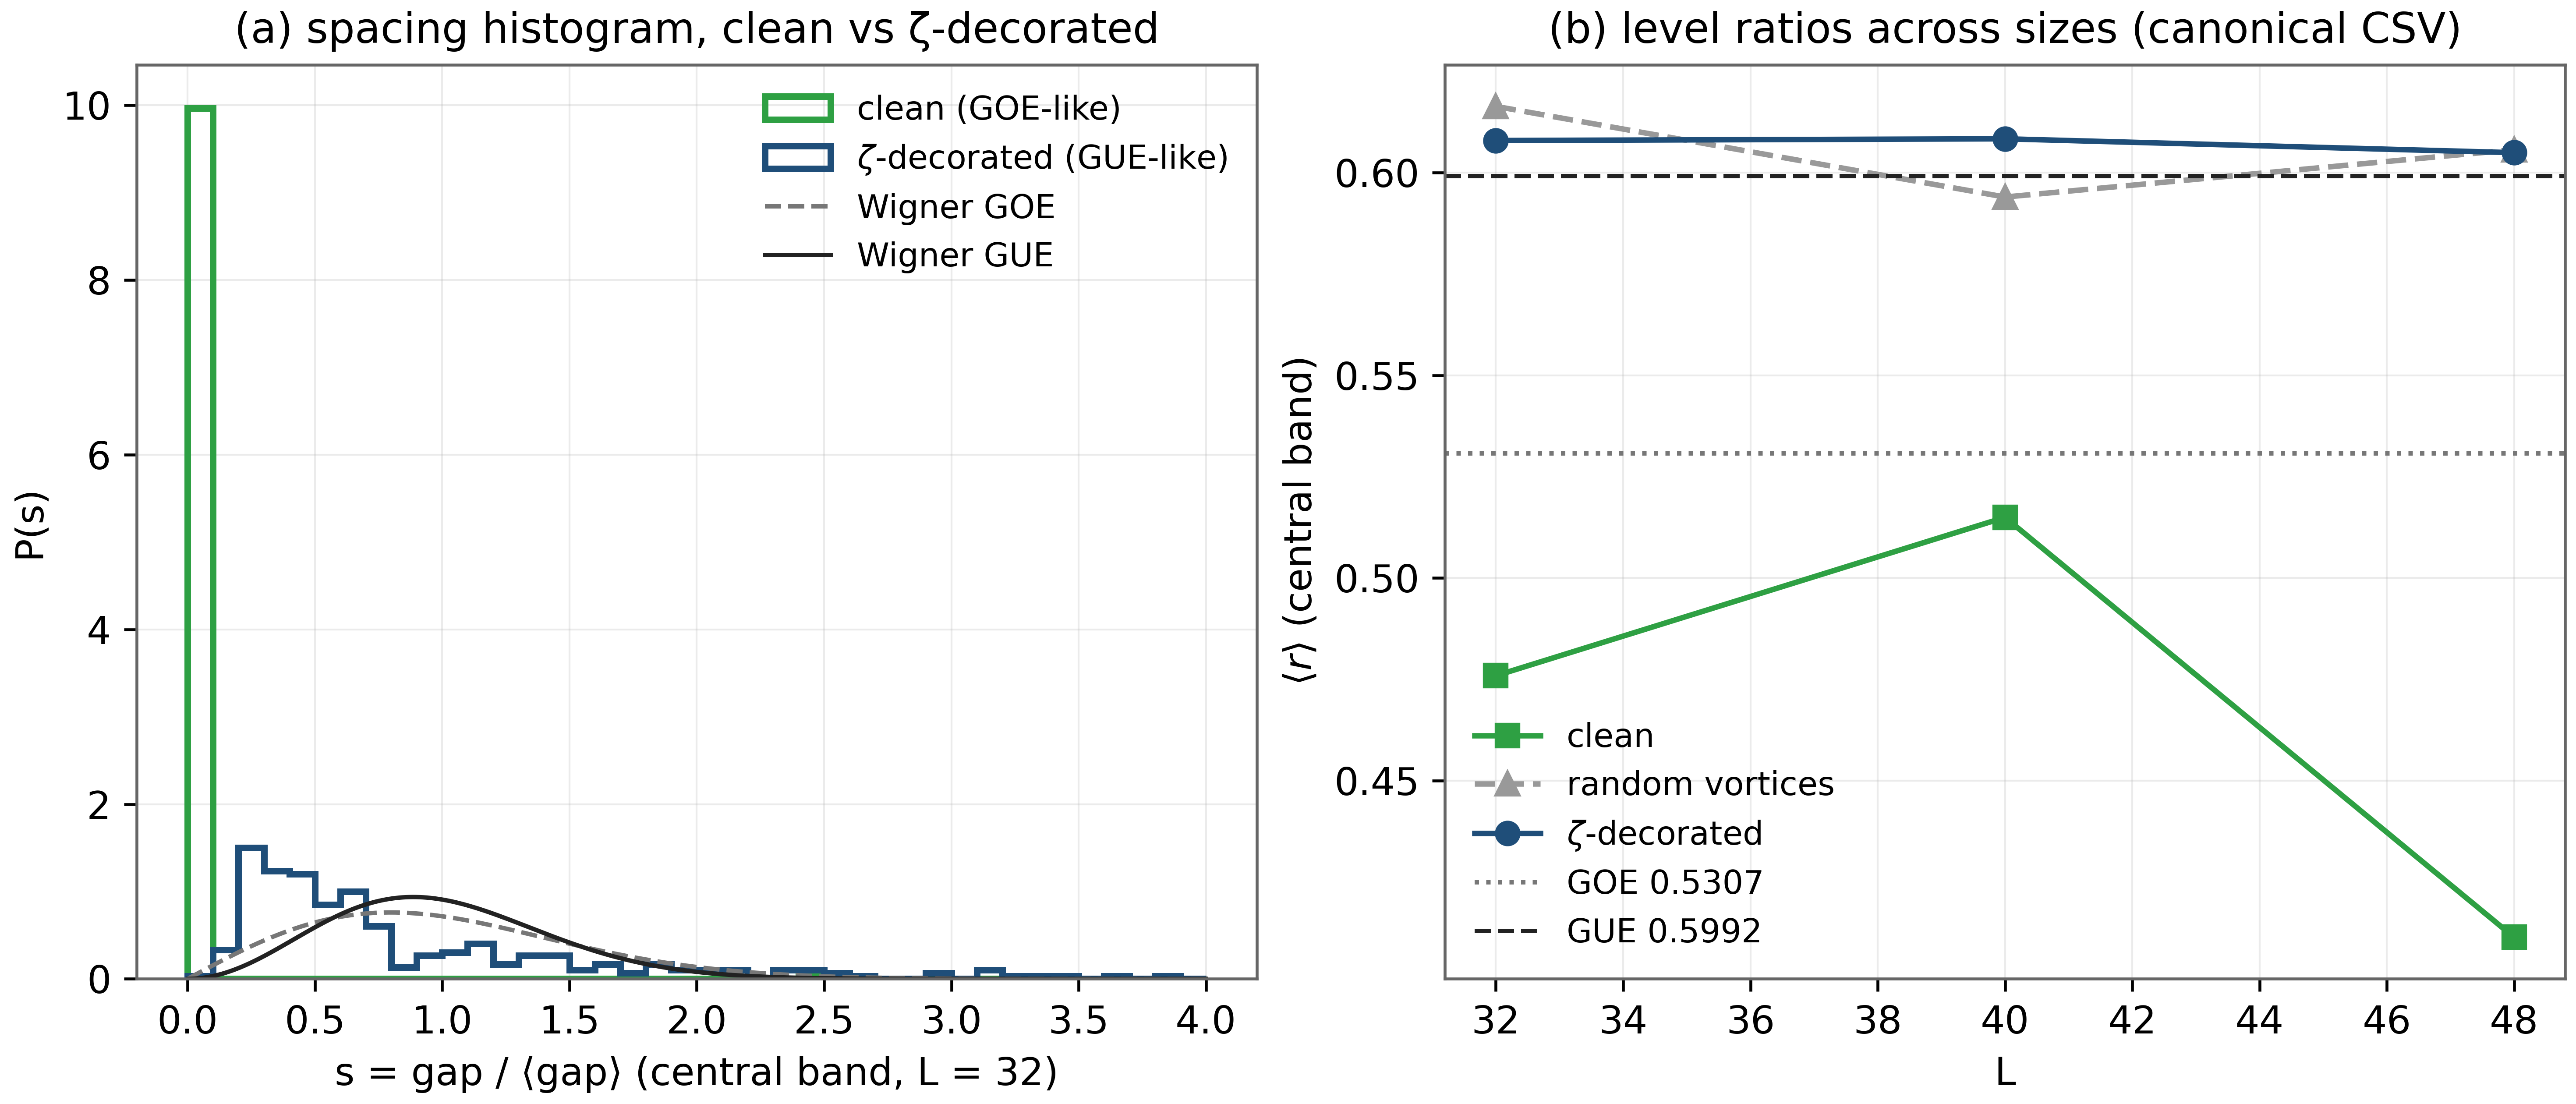
\includegraphics[max width=\columnwidth, max height=0.42\textheight]{figures/d07_extra_statistics.png}
\caption{Companion panels: (a) central-band spacing histogram $P(s)$, clean vs $\zeta$-decorated at $L=32$, against the Wigner GOE/GUE surmises (recomputed); (b) the canonical CSV ladder of $\langle r\rangle$ with GOE/GUE reference lines.}\label{fig:d7_2}
\end{figure}

\section{Discussion}
D7 is the intellectual hinge of the laboratory. Its positive half -- the GUE lift -- shows that the zeros' arithmetic is strong enough to reorganize the spectral statistics of a certified Dirac operator, which is the operational content of the parent programme's bridge. Its negative half is equally important: it draws the boundary of what the decoration cannot do, and that boundary is what makes D9's constructive answer (index restoration through a Jackiw--Rossi wall) meaningful rather than rhetorical \cite{jackiwrebbi}.

Methodologically the test demonstrates that unfolding-free statistics ($\langle r\rangle$) are the right observables for lattice spectra with unknown density renormalization; the companion $P(s)$ panel shows the same story in histogram form. Extensions should keep this discipline: any new decoration should be scored on $\langle r\rangle$ \emph{and} on the symmetry audit before any sharper claim is made.

\section{Reproducibility}
\begin{itemize}[leftmargin=1.2em, itemsep=0.15em]
\item \textbf{Single test:} \texttt{python3} \path{code/dirac_lab.py} \texttt{--test D7} (add \texttt{--quick} for a reduced pass; \texttt{--no-figures} to skip the 600-dpi figure).
\item \textbf{Canonical run:} \texttt{make all} regenerates the whole D1--D14 ledger into \path{results/}; this monograph's ledger is the verbatim per-check table of that run.
\item \textbf{Determinism:} seed 96 (parent convention); the $\zeta$ tables are the Odlyzko-derived files in \path{data/} with provenance in their headers.
\item \textbf{Figures:} the canonical figure was regenerated into this folder by the v1.4 harness (the original test function itself); companion panels are recomputed with the same modules (\path{scripts/make_extra_figures.py}). All figures are 600 dpi.
\item \textbf{Cross-verification:} \texttt{julia} \path{code/dirac_lab_cross.jl} re-derives this test's verdicts from the written conventions alone (see \path{results/CROSS_VERIFICATION.md}).
\item \textbf{Artifacts in this folder:} \path{monograph.tex} (this document's source), \path{results.json} (machine-readable ledger), \path{figures/} (600-dpi figures), and the canonical CSV of the test.
\end{itemize}

\section*{References}
\begin{thebibliography}{99}\small
\bibitem{parent} I. K. Isaev, AB-Cloud Research: the Hofstadter--Aharonov--Bohm realization of the Hilbert--P'olya programme (parent repository and test ledger), \url{https://github.com/wild8highlander/ab-cloud-research} (2026).
\bibitem{ab} Y. Aharonov and D. Bohm, Significance of electromagnetic potentials in the quantum theory, Phys. Rev. 115, 485 (1959).
\bibitem{guhr} T. Guhr, A. M"uller-Groeling, and H. A. Weidenm"uller, Random-matrix theories in quantum physics: common concepts, Phys. Rep. 299, 189 (1998).
\bibitem{mehta} M. L. Mehta, Random Matrices, 3rd ed. (Elsevier/Academic Press, 2004).
\bibitem{riemannvm} B. Riemann (1859); H. von Mangoldt, Zu Riemanns Abhandlung ``Ueber die Anzahl der Primzahlen unter einer gegebenen Gr"osse'', J. reine angew. Math. 114, 255 (1895).
\bibitem{atyahbott} M. F. Atiyah and R. Bott, The Yang--Mills equations over Riemann surfaces, Philos. Trans. R. Soc. A 308, 523 (1983).
\bibitem{jackiwrebbi} R. Jackiw and C. Rebbi, Solitons with fermion number $1/2$, Phys. Rev. D 13, 3398 (1976).
\end{thebibliography}

\vfill
\noindent\rule{\textwidth}{0.4pt}\\[0.2em]
{\footnotesize\color{labgray} AB-Cloud Dirac Laboratory · per-test monograph series v1.4 · compiled with Tectonic (LaTeX) · all numbers traceable to \texttt{results/run\_20261006\_full\_v13} · \texttt{D7} of 14.}

\end{document}